% \documentclass[a4paper,12pt,francais,twoside,openright]{article}
% \usepackage[french]{babel}
% \usepackage[left=1.5cm, right=1cm, top=1.5cm, bottom=1.5cm]{geometry}
% \usepackage{ProfCollege}
% \usepackage{ProfMaquette}
% \usepackage{OutilsGeomTikz}
% \usepackage{enumitem}
% \usepackage{PanneauxRoute}
% \usetikzlibrary{decorations.pathmorphing}
% \usepackage{fancyhdr}
% \usepackage{postit}
% \pagestyle{fancy}
% \AtEndDocument{\label{lastpage}}
% \fancyfoot[CE,CO]{Symétrie centrale -- page \thepage ~sur \pageref{lastpage}}
% \fancyhead[CE,CO,LE,LO,RE,RO]{}
% \renewcommand{\headrulewidth}{0pt}
% \renewcommand{\footrulewidth}{0.4pt}
%
%
%
% \begin{document}
\begin{Maquette}[Fiche]{Niveau=5\ieme{},Classe={},Date={},Theme=Symétrie centrale,NomExercice=Activité}
%
%
%
\begin{exercice}

\MultiCol{0.6/0.3}{
	On va construire l'image de la figure par la symétrie de centre $O$.
§
	\begin{PostIt}
		\textbf{ATTENTION} c'est différent de la symétrie axiale que tu connais déjà !
	\end{PostIt}
}
	
	\MultiCol{0.45/0.45}{
			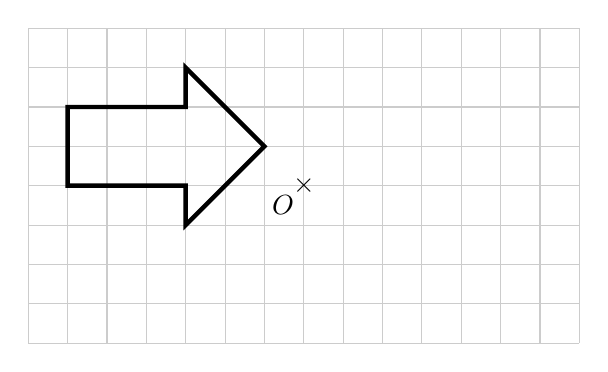
\begin{tikzpicture}[scale=0.5]
				\draw[gray!40] (0,0) grid (14,8);
					\draw [ultra thick] (1,4)--(4,4)--(4,3)--(6,5)--(4,7)--(4,6)--(1,6)--cycle;
					\draw (7,4) node{$\times$} node[below left]{$O$};
			\end{tikzpicture}
§
		\begin{center}
		\textbf{\'Etape 1:}
		\end{center}
		On va regarder le \og{} \textit{chemin} \fg{} du point $A$ au point $O$.
		
			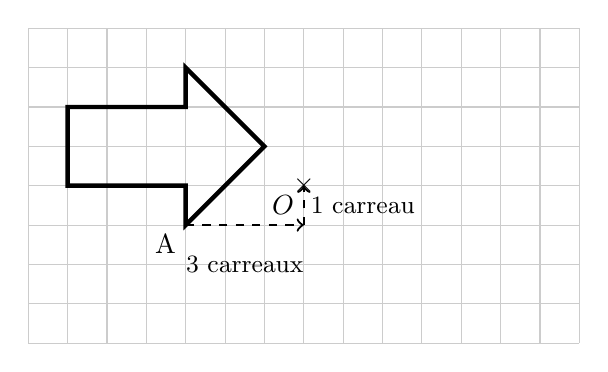
\begin{tikzpicture}[scale=0.5]
				\draw[gray!40] (0,0) grid (14,8);
					\draw [ultra thick] (1,4)--(4,4)--(4,3)--(6,5)--(4,7)--(4,6)--(1,6)--cycle;
					\draw (4,3) node[below left]{A};
					\draw[dashed, thick,->] (4,3)--(7,3); 
					\draw (5.5,2) node{\small 3 carreaux};
					\draw[dashed, thick,->] (7,3)--(7,4);
					\draw (8.5,3.5) node{\small 1 carreau};
					\draw (7,4) node{$\times$} node[below left]{$O$};
			\end{tikzpicture}
	}

\MultiCol{0.45/0.45}{
		\begin{center}
		\textbf{\'Etape 2:}
		\end{center}
		On exécute le même \og{} \textit{chemin} \fg{}, cette fois en partant du point $O$. On trouve alors le point $A'$, image du point $A$ par la symétrie de centre $O$.
		
			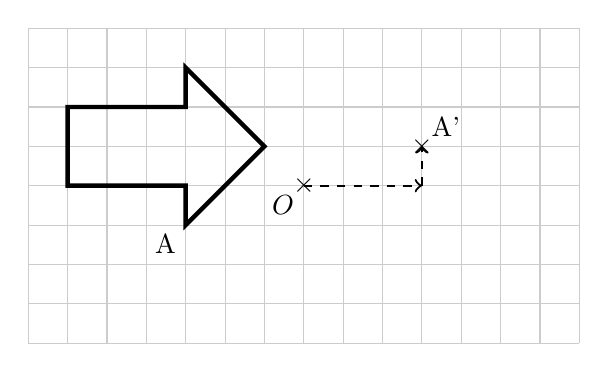
\begin{tikzpicture}[scale=0.5]
				\draw[gray!40] (0,0) grid (14,8);
					\draw [ultra thick] (1,4)--(4,4)--(4,3)--(6,5)--(4,7)--(4,6)--(1,6)--cycle;
					\draw (4,3) node[below left]{A};
					\draw[dashed, thick,->] (7,4)--(10,4); 
%					\draw (5.5,2) node{3 carreaux};
					\draw[dashed, thick,->] (10,4)--(10,5);
%					\draw (8.5,3.5) node{1 carreau};
					\draw (7,4) node{$\times$} node[below left]{$O$};
					\draw (10,5) node{$\times$} node[above right]{A'};
			\end{tikzpicture}
§
		\begin{center}
		\textbf{\'Etape 4:}
		\end{center}
		Fait de même avec les autres points de la figure de façon à obtenir l'image de la flèche par la symétrie de centre $O$.
		
			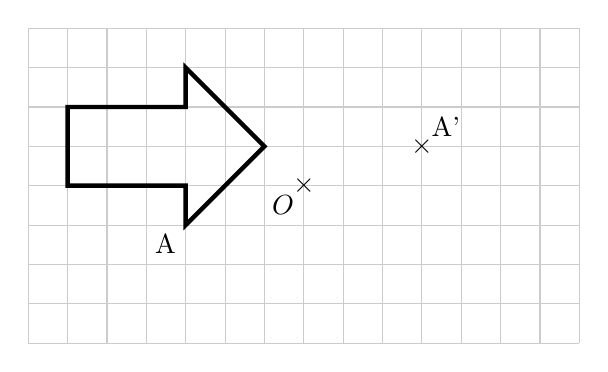
\begin{tikzpicture}[scale=0.5]
				\draw[gray!40] (0,0) grid (14,8);
					\draw [ultra thick] (1,4)--(4,4)--(4,3)--(6,5)--(4,7)--(4,6)--(1,6)--cycle;
					\draw (4,3) node[below left]{A};
					\draw (7,4) node{$\times$} node[below left]{$O$};
					\draw (10,5) node{$\times$} node[above right]{A'};
			\end{tikzpicture}			
}
\end{exercice}

\begin{exercice}
\MultiCol{0.45/0.45}{
\begin{enumerate}
	\item Construis l'image de la figure par la symétrie de centre $O$.
	\item En analysant la figure obtenue dans cette exercice ainsi que dans le précédent, comment décrirais-tu cette nouvelle transformation ?
\end{enumerate}
\Lignespointilles{5}
§
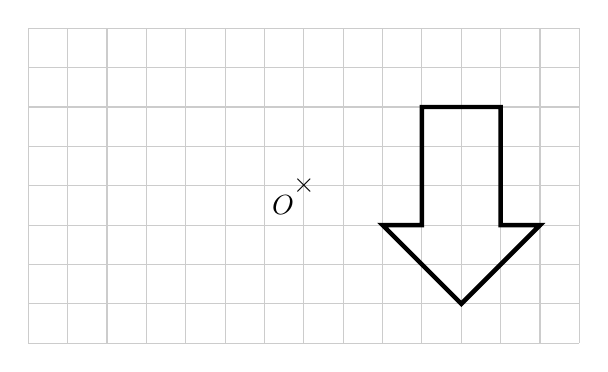
\begin{tikzpicture}[scale=0.5]
	\draw[gray!40] (0,0) grid (14,8);
	\draw [ultra thick] (11,1)--(13,3)--(12,3)--(12,6)--(10,6)--(10,3)--(9,3)--cycle;
	\draw (7,4) node{$\times$} node[below left]{$O$};
\end{tikzpicture}
}
\end{exercice}

\begin{exercice}


\MultiCol{0.4/0.5}{
\begin{enumerate}
	\item Dans chaque cas, construis l'image de la figure par la symétrie de centre $O$ :
\end{enumerate}
	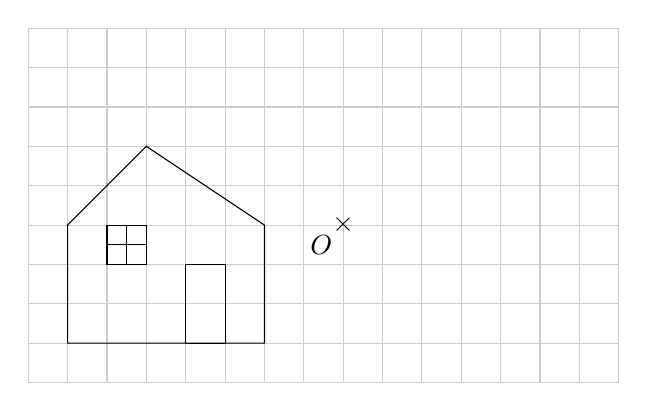
\begin{tikzpicture}[scale=0.5]
		\draw [gray!40] (-6,-1) grid (9,8);
		\draw[very thick] (2,3) node{$\times$} node[below left]{$O$};
			\draw (0,0)--(-5,0)--(-5,3)--(-3,5)--(0,3)--cycle;
			\draw (-2,0)rectangle (-1,2);
			\draw (-4,2) rectangle (-3,3);
			\draw (-3.5,2)--(-3.5,3);
			\draw (-4,2.5)--(-3,2.5);
	\end{tikzpicture}
§
\begin{enumerate}[start=2]
	\item Construis l'image du nombre \textbf{$\num{713705}$} par la symétrie de centre $O$.
\end{enumerate}
	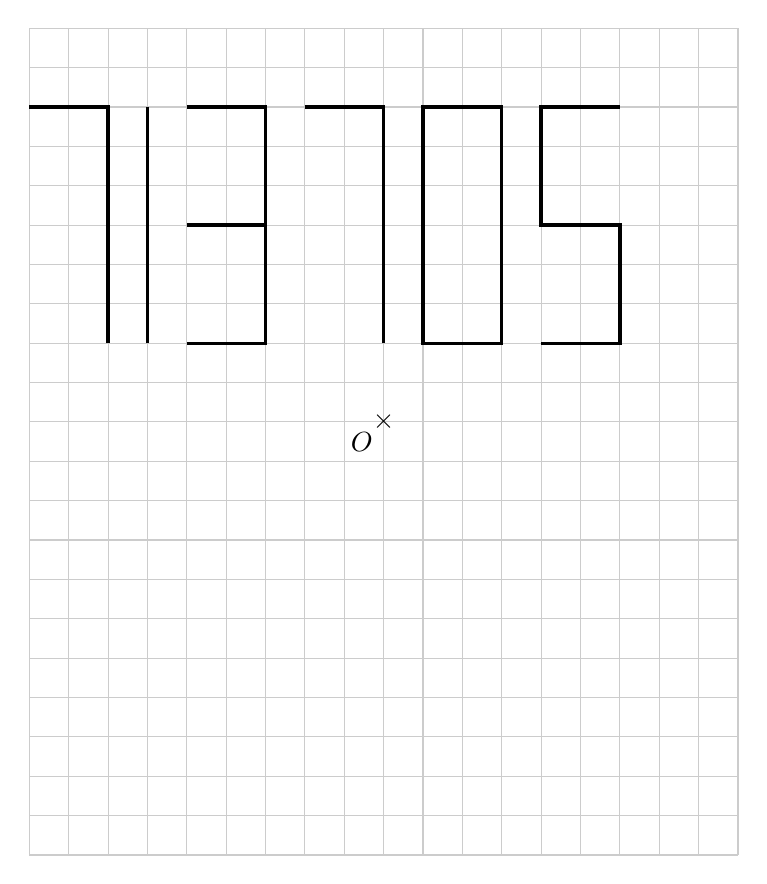
\begin{tikzpicture}[scale=0.5]
		\draw [gray!40] (0,0) grid (18,21);
		\draw[very thick] (9,11) node{$\times$} node[below left]{$O$};
			\draw[very thick] (2,13)--(2,19)--(0,19);
			\draw[very thick] (3,13)--(3,19);
			\draw[very thick] (4,13)--(6,13)--(6,19)--(4,19);
			\draw[very thick] (4,16)--(6,16);
			\draw[very thick] (9,13)--(9,19)--(7,19);
			\draw[very thick] (10,13)rectangle(12,19);
			\draw[very thick] (13,13)--(15,13)--(15,16)--(13,16)--(13,19)--(15,19);
	\end{tikzpicture}
}
\end{exercice}
%
%
%
\begin{exercice}[Source=Coopmaths]
\begin{center}
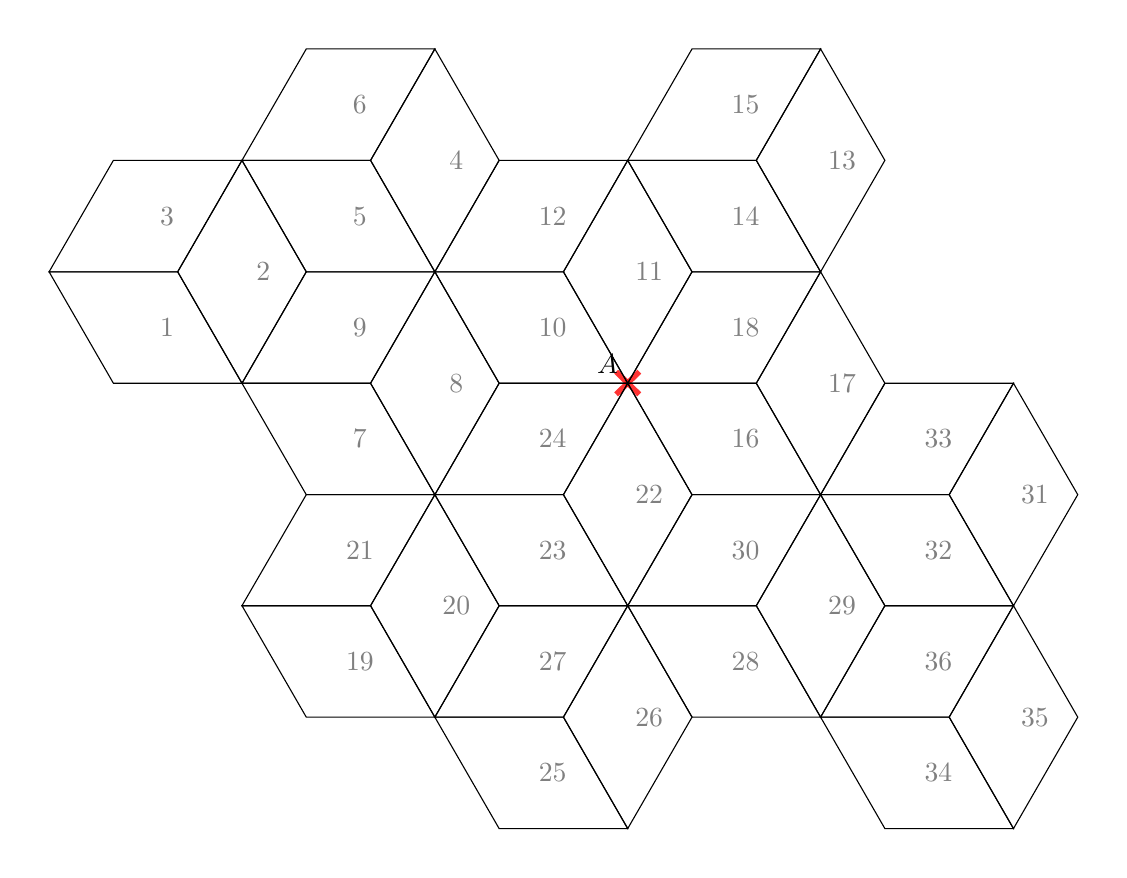
\begin{tikzpicture}[baseline,scale = 0.5443310539518174]

    \tikzset{
      point/.style={
        thick,
        draw,
        cross out,
        inner sep=0pt,
        minimum width=5pt,
        minimum height=5pt,
      },
    }
    \clip (-0.5,-13.490381056766577) rectangle (24.5,5.696152422706633);


    	
	\draw[color ={{red}},line width = 2,opacity = 0.8] (13.23,-2.33)--(13.77,-2.86);
	\draw[color ={{red}},line width = 2,opacity = 0.8] (13.23,-2.86)--(13.77,-2.33);
		\draw (13.5,-2.6) node[above left] {$A$};

	\draw [color={gray},fill opacity = 1] (2.75,-1.3) node[anchor = center,scale=1] {$1$};
	\draw [color={gray},fill opacity = 1] (5,0) node[anchor = center,scale=1] {$2$};
	\draw [color={gray},fill opacity = 1] (2.75,1.3) node[anchor = center,scale=1] {$3$};
	\draw [color={gray},fill opacity = 1] (9.5,2.6) node[anchor = center,scale=1] {$4$};
	\draw [color={gray},fill opacity = 1] (7.25,1.3) node[anchor = center,scale=1] {$5$};
	\draw [color={gray},fill opacity = 1] (7.25,3.9) node[anchor = center,scale=1] {$6$};
	\draw [color={gray},fill opacity = 1] (7.25,-3.9) node[anchor = center,scale=1] {$7$};
	\draw [color={gray},fill opacity = 1] (9.5,-2.6) node[anchor = center,scale=1] {$8$};
	\draw [color={gray},fill opacity = 1] (7.25,-1.3) node[anchor = center,scale=1] {$9$};
	\draw [color={gray},fill opacity = 1] (11.75,-1.3) node[anchor = center,scale=1] {$10$};
	\draw [color={gray},fill opacity = 1] (14,0) node[anchor = center,scale=1] {$11$};
	\draw [color={gray},fill opacity = 1] (11.75,1.3) node[anchor = center,scale=1] {$12$};
	\draw [color={gray},fill opacity = 1] (18.5,2.6) node[anchor = center,scale=1] {$13$};
	\draw [color={gray},fill opacity = 1] (16.25,1.3) node[anchor = center,scale=1] {$14$};
	\draw [color={gray},fill opacity = 1] (16.25,3.9) node[anchor = center,scale=1] {$15$};
	\draw [color={gray},fill opacity = 1] (16.25,-3.9) node[anchor = center,scale=1] {$16$};
	\draw [color={gray},fill opacity = 1] (18.5,-2.6) node[anchor = center,scale=1] {$17$};
	\draw [color={gray},fill opacity = 1] (16.25,-1.3) node[anchor = center,scale=1] {$18$};
	\draw [color={gray},fill opacity = 1] (7.25,-9.09) node[anchor = center,scale=1] {$19$};
	\draw [color={gray},fill opacity = 1] (9.5,-7.79) node[anchor = center,scale=1] {$20$};
	\draw [color={gray},fill opacity = 1] (7.25,-6.5) node[anchor = center,scale=1] {$21$};
	\draw [color={gray},fill opacity = 1] (14,-5.2) node[anchor = center,scale=1] {$22$};
	\draw [color={gray},fill opacity = 1] (11.75,-6.5) node[anchor = center,scale=1] {$23$};
	\draw [color={gray},fill opacity = 1] (11.75,-3.9) node[anchor = center,scale=1] {$24$};
	\draw [color={gray},fill opacity = 1] (11.75,-11.69) node[anchor = center,scale=1] {$25$};
	\draw [color={gray},fill opacity = 1] (14,-10.39) node[anchor = center,scale=1] {$26$};
	\draw [color={gray},fill opacity = 1] (11.75,-9.09) node[anchor = center,scale=1] {$27$};
	\draw [color={gray},fill opacity = 1] (16.25,-9.09) node[anchor = center,scale=1] {$28$};
	\draw [color={gray},fill opacity = 1] (18.5,-7.79) node[anchor = center,scale=1] {$29$};
	\draw [color={gray},fill opacity = 1] (16.25,-6.5) node[anchor = center,scale=1] {$30$};
	\draw [color={gray},fill opacity = 1] (23,-5.2) node[anchor = center,scale=1] {$31$};
	\draw [color={gray},fill opacity = 1] (20.75,-6.5) node[anchor = center,scale=1] {$32$};
	\draw [color={gray},fill opacity = 1] (20.75,-3.9) node[anchor = center,scale=1] {$33$};
	\draw [color={gray},fill opacity = 1] (20.75,-11.69) node[anchor = center,scale=1] {$34$};
	\draw [color={gray},fill opacity = 1] (23,-10.39) node[anchor = center,scale=1] {$35$};
	\draw [color={gray},fill opacity = 1] (20.75,-9.09) node[anchor = center,scale=1] {$36$};
	\draw[color={black}] (0,0)--(3,0)--(4.5,-2.6)--(1.5,-2.6)--cycle;
	\draw[color={black}] (4.5,2.6)--(6,0)--(4.5,-2.6)--(3,0)--cycle;
	\draw[color={black}] (0,0)--(1.5,2.6)--(4.5,2.6)--(3,0)--cycle;
	\draw[color={black}] (9,5.2)--(10.5,2.6)--(9,0)--(7.5,2.6)--cycle;
	\draw[color={black}] (4.5,2.6)--(7.5,2.6)--(9,0)--(6,0)--cycle;
	\draw[color={black}] (4.5,2.6)--(6,5.2)--(9,5.2)--(7.5,2.6)--cycle;
	\draw[color={black}] (4.5,-2.6)--(7.5,-2.6)--(9,-5.2)--(6,-5.2)--cycle;
	\draw[color={black}] (9,0)--(10.5,-2.6)--(9,-5.2)--(7.5,-2.6)--cycle;
	\draw[color={black}] (4.5,-2.6)--(6,0)--(9,0)--(7.5,-2.6)--cycle;
	\draw[color={black}] (9,0)--(12,0)--(13.5,-2.6)--(10.5,-2.6)--cycle;
	\draw[color={black}] (13.5,2.6)--(15,0)--(13.5,-2.6)--(12,0)--cycle;
	\draw[color={black}] (9,0)--(10.5,2.6)--(13.5,2.6)--(12,0)--cycle;
	\draw[color={black}] (18,5.2)--(19.5,2.6)--(18,0)--(16.5,2.6)--cycle;
	\draw[color={black}] (13.5,2.6)--(16.5,2.6)--(18,0)--(15,0)--cycle;
	\draw[color={black}] (13.5,2.6)--(15,5.2)--(18,5.2)--(16.5,2.6)--cycle;
	\draw[color={black}] (13.5,-2.6)--(16.5,-2.6)--(18,-5.2)--(15,-5.2)--cycle;
	\draw[color={black}] (18,0)--(19.5,-2.6)--(18,-5.2)--(16.5,-2.6)--cycle;
	\draw[color={black}] (13.5,-2.6)--(15,0)--(18,0)--(16.5,-2.6)--cycle;
	\draw[color={black}] (4.5,-7.79)--(7.5,-7.79)--(9,-10.39)--(6,-10.39)--cycle;
	\draw[color={black}] (9,-5.2)--(10.5,-7.79)--(9,-10.39)--(7.5,-7.79)--cycle;
	\draw[color={black}] (4.5,-7.79)--(6,-5.2)--(9,-5.2)--(7.5,-7.79)--cycle;
	\draw[color={black}] (13.5,-2.6)--(15,-5.2)--(13.5,-7.79)--(12,-5.2)--cycle;
	\draw[color={black}] (9,-5.2)--(12,-5.2)--(13.5,-7.79)--(10.5,-7.79)--cycle;
	\draw[color={black}] (9,-5.2)--(10.5,-2.6)--(13.5,-2.6)--(12,-5.2)--cycle;
	\draw[color={black}] (9,-10.39)--(12,-10.39)--(13.5,-12.99)--(10.5,-12.99)--cycle;
	\draw[color={black}] (13.5,-7.79)--(15,-10.39)--(13.5,-12.99)--(12,-10.39)--cycle;
	\draw[color={black}] (9,-10.39)--(10.5,-7.79)--(13.5,-7.79)--(12,-10.39)--cycle;
	\draw[color={black}] (13.5,-7.79)--(16.5,-7.79)--(18,-10.39)--(15,-10.39)--cycle;
	\draw[color={black}] (18,-5.2)--(19.5,-7.79)--(18,-10.39)--(16.5,-7.79)--cycle;
	\draw[color={black}] (13.5,-7.79)--(15,-5.2)--(18,-5.2)--(16.5,-7.79)--cycle;
	\draw[color={black}] (22.5,-2.6)--(24,-5.2)--(22.5,-7.79)--(21,-5.2)--cycle;
	\draw[color={black}] (18,-5.2)--(21,-5.2)--(22.5,-7.79)--(19.5,-7.79)--cycle;
	\draw[color={black}] (18,-5.2)--(19.5,-2.6)--(22.5,-2.6)--(21,-5.2)--cycle;
	\draw[color={black}] (18,-10.39)--(21,-10.39)--(22.5,-12.99)--(19.5,-12.99)--cycle;
	\draw[color={black}] (22.5,-7.79)--(24,-10.39)--(22.5,-12.99)--(21,-10.39)--cycle;
	\draw[color={black}] (18,-10.39)--(19.5,-7.79)--(22.5,-7.79)--(21,-10.39)--cycle;

\end{tikzpicture}
\end{center}

Quelle est l'image de la figure $2$ dans la symétrie de centre $A$ ?

Quelle est l'image de la figure $18$ dans la symétrie de centre $A$ ?

Quelle est l'image de la figure $9$ dans la symétrie de centre $A$ ?

Quelle est l'image de la figure $6$ dans la symétrie de centre $A$ ?

Quelle est l'image de la figure $12$ dans la symétrie de centre $A$ ?
\end{exercice}
%
%
%
\newpage
%
%
%
\begin{tcolorbox}[title=Avec les instruments de géométrie (exemples)]
On construit le point $A'$, image du point $A$ par la symétrie de centre $O$.

\MultiCol{0.22/0.22/0.22/0.22}{
	\begin{center}
		\textbf{\'Enoncé :}
	\end{center}
§
	\begin{center}
		\textbf{\'Etape 1:}
	\end{center}
	Trace la demi-droite $[AO)$ en pointillés.
§	
	\begin{center}
		\textbf{\'Etape 2:}
	\end{center}
	Plante le compas en $O$, prendre l'écart entre $O$ et $A$.
§
	\begin{center}
		\textbf{\'Etape 3:}
	\end{center}
	Reporte la longueur de l'autre côté du point $O$.
}
	
\MultiCol{0.22/0.22/0.22/0.22}{
			\begin{tikzpicture}[scale=0.5]
			\clip (-4,-5) rectangle (4,5);
				\draw[ultra thick] (0,0) node{$\times$} node[below left]{$O$};
				\draw (-3,-2) node{$\times$} node[below left]{$A$};
			\end{tikzpicture}
§
			\begin{tikzpicture}[scale=0.5]
			\clip (-4,-5) rectangle (4,5);
				\draw[ultra thick] (0,0) node{$\times$} node[below left]{$O$};
				\draw (-3,-2) node{$\times$} node[below left]{$A$};
				\draw[dashed] plot[domain=-3:3.5] (\x,2*\x/3);
			\end{tikzpicture}
§
			\begin{tikzpicture}[scale=0.5]
			\clip (-4,-5) rectangle (4,5);
			\coordinate (O) at (0,0);
			\coordinate (A) at (-3,-2);
				\draw[ultra thick] (0,0) node{$\times$} node[below left]{$O$};
				\draw (-3,-2) node{$\times$} node[below left]{$A$};
				\draw[dashed] plot[domain=-3:3.5] (\x,2*\x/3);
				\tkzCompas[Echelle=0.75]{O}{A};
			\end{tikzpicture}
§
			\begin{tikzpicture}[scale=0.5]
			\clip (-4,-5) rectangle (4,5);
			\coordinate (O) at (0,0);
			\coordinate (A') at (3,2);
				\draw[ultra thick] (0,0) node{$\times$} node[below left]{$O$};
				\draw (-3,-2) node{$\times$} node[below left]{$A$};
				\draw[dashed] plot[domain=-3:3.5] (\x,2*\x/3);
				\tkzCompas[Echelle=0.75]{O}{A'};
				\draw (A') node{$\times$} node[below right]{$A'$};
			\end{tikzpicture}
}
\end{tcolorbox}

\begin{exercice}
\MultiCol{0.45/0.45}{
\begin{enumerate}
	\item Construis l'image du triangle $ABC$ par la symétrie de centre $O$ en utilisant ton compas.
\end{enumerate}


\begin{center}
	\begin{tikzpicture}[scale=0.65]
		\draw (0,0) node{$\times$}node[below left]{$O$};
			\draw (-3,-2) node[below left]{$A$};
			\draw (-5,0) node[left]{$B$};
			\draw (-2,2) node[above]{$C$};
				\draw[ultra thick] (-3,-2)--(-5,0)--(-2,2)--cycle;
					\draw[dashed] plot[domain=-5:7] (\x,0);
					\draw[dashed] plot[domain=-3:5] (\x,2*\x/3);
					\draw[dashed] plot[domain=-2:4] (\x,-1*\x);
	\end{tikzpicture}
\end{center}
§
\begin{enumerate}[resume]
	\item Construis l'image du triangle $ABC$ par la symétrie de centre $O$ en utilisant ta règle.
\end{enumerate}


\begin{center}
	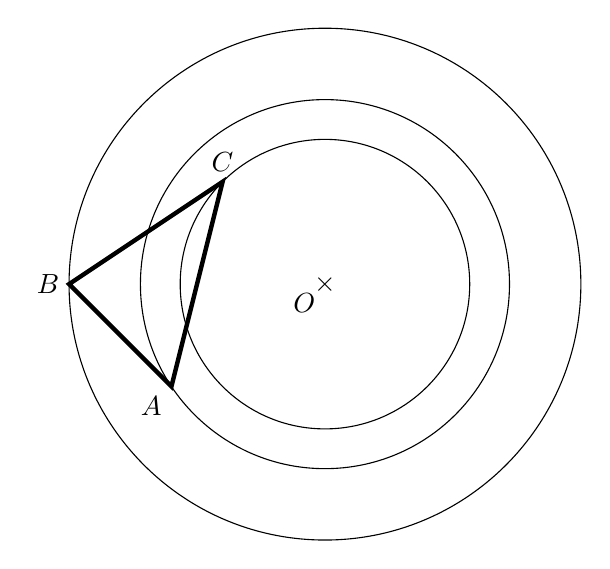
\begin{tikzpicture}[scale=0.65]
		\draw (0,0) node{$\times$}node[below left]{$O$};
			\draw (-3,-2) node[below left]{$A$};
			\draw (-5,0) node[left]{$B$};
			\draw (-2,2) node[above]{$C$};
				\draw[ultra thick] (-3,-2)--(-5,0)--(-2,2)--cycle;
					\draw (0,0) circle(5);
					\draw (0,0) circle(2.828427);
					\draw (0,0) circle(3.60555);
	\end{tikzpicture}
\end{center}
}
\end{exercice}

\begin{exercice}[Source=Cahier Sesamaths édition 2021]

\MultiCol{0.45/0.45}{
\begin{enumerate}
	\item Construis l'image du triangle $ABC$ par la symétrie de centre $A$. Tu appelles cette figure la figure 1.
	\item Construis l'image du triangle $ABC$ par la symétrie de centre $P$. Tu appelles cette figure la figure 2.
	\item Construis l'image du triangle $ABC$ par la symétrie de centre $L$. Tu appelles cette figure la figure 3.
\end{enumerate}
§
\begin{center}
	\begin{tikzpicture}[scale=0.75]
		\clip (-6,-3)rectangle(3,6.5);
			\draw[ultra thick] (-2,2)--(1,1)--(-1,-2)--cycle;
			\draw (-1,0) node{$\times$}node[below left]{$L$};
			\draw (0.39,1.22) node{$\times$}node[below left]{$P$};
			\draw (-2,2) node[above left]{$A$};
			\draw (1,1) node[above right]{$B$};
			\draw (-1,-2) node[below right]{$C$};
	\end{tikzpicture}
\end{center}
}
\end{exercice}

\begin{exercice}[Source=Cahier Sesamaths édition 2021]
Construis l'image du chien par la symétrie de centre $O$.
\begin{center}
	\begin{tikzpicture}
		\clip (-7,-5) rectangle (7,5);
			\draw (0,0) node{$\times$} node[above right]{$O$};
			\draw[ultra thick] (-3,3)--(-2,1)--(3,2)--(4,4)--(4,3)--(6.5,2)--(6,1)--(4,0.5)--(3,-3)--(2,-1)--(-1,-1)--(-2,-3)--(-2,0)--cycle;
			\draw[fill=black] (4.2,2) circle(0.1);
	\end{tikzpicture}
\end{center}
\end{exercice}

\begin{exercice}
	Pour chacun des panneaux ci-dessous, marque, s'ils existent, le ou les centres de symétrie.
	
	\prLimVites{80} \hfill \prChausRet \hfill \prDeuxSens \hfill \prRoutePrio \hfill \prRondPoint \hfill \prCircInterd \hfill \prSensInterdit \hfill \prStationInterd \hfill \prObliAvDroite \hfill \prObliDroiteGauche \hfill \prObliChaines \hfill \prFinInterd
\end{exercice}


\end{Maquette}

% \end{document}